\documentclass[12pt, a4paper]{article}

% ==================== 中文与字体 ====================
\usepackage{fontspec}
\usepackage{xeCJK}
\setCJKmainfont{仿宋}[AutoFakeBold=true, AutoFakeSlant=true]
\setmainfont{Cambria}

% ==================== 页面布局 ====================
\usepackage{geometry}
\geometry{
    a4paper,
    left=2.8cm,
    right=2.8cm,
    top=2.8cm,
    bottom=2.8cm,
    headheight=15pt
}

% ==================== 颜色系统 ====================
\usepackage{xcolor}
\definecolor{mainblue}{RGB}{0, 182, 255}
\definecolor{lightblue}{RGB}{200, 220, 240}
\definecolor{codegray}{RGB}{245, 245, 245}
\definecolor{keywordcolor}{RGB}{0, 0, 255}
\definecolor{stringcolor}{RGB}{163, 21, 21}
\definecolor{commentcolor}{RGB}{0, 128, 0}

% ==================== 页眉页脚 ====================
\usepackage{fancyhdr}
\pagestyle{fancy}
\fancyhf{}
\renewcommand{\headrulewidth}{0.8pt}
\renewcommand{\headrule}{\color{mainblue}\hrule width\textwidth height 0.8pt}
\fancyhead[L]{\textcolor{mainblue}{\textbf{系统开发工具基础 · Week 1}}}
\fancyhead[R]{\textcolor{mainblue}{\thepage}}
\fancyfoot[C]{\textcolor{gray}{\small 25020007096 · Xingrui Pan}}

% ==================== 章节标题样式 ====================
\usepackage{titlesec, titletoc}
\titleformat{\section}
    {\Large\bfseries\color{mainblue}}
    {\thesection}{1em}{}
    [{\titlerule[0.5pt]}]

\titleformat{\subsection}
    {\large\bfseries\color{mainblue!80!black}}
    {\thesubsection}{1em}{}

% ==================== 目录样式 ====================
\usepackage{tocloft}
\renewcommand{\cftsecfont}{\color{mainblue}\bfseries}
\renewcommand{\cftsubsecfont}{\color{mainblue!80!black}}
\renewcommand{\cftsecpagefont}{\color{mainblue}}

% ==================== 列表样式 ====================
\usepackage{enumitem}
\setlist[enumerate]{
    label=\color{mainblue}\arabic*.,
    ref=\arabic*,
    leftmargin=1.2cm,
    itemsep=2pt
}
\setlist[itemize]{
    label=\textcolor{mainblue}{\textbullet},
    leftmargin=1.2cm,
    itemsep=2pt
}

% ==================== 图表与浮动体 ====================
\usepackage{graphicx}
\usepackage{caption}
\usepackage{subcaption}
\usepackage{float}
\captionsetup{
    font=small,
    labelfont={bf,color=mainblue},
    labelsep=period
}

% ==================== 表格增强 ====================
\usepackage{array, booktabs, colortbl}
\newcolumntype{C}{>{\centering\arraybackslash}X}

% ==================== 代码高亮 ====================
\usepackage{listings}
\lstset{
    basicstyle=\ttfamily\small,
    keywordstyle=\color{keywordcolor}\bfseries,
    stringstyle=\color{stringcolor},
    commentstyle=\color{commentcolor}\itshape,
    backgroundcolor=\color{codegray},
    frame=single,
    frameround=tttt,
    framesep=5pt,
    breaklines=true,
    showspaces=false,
    showstringspaces=false,
    tabsize=4,
    numbers=left,
    numberstyle=\tiny\color{gray},
    captionpos=b,
    xleftmargin=2pt,
    xrightmargin=2pt
}

% ==================== 数学公式 ====================
\usepackage{amsmath, amssymb, bm}
\usepackage{mathtools}
\numberwithin{equation}{section}

% ==================== 超链接 ====================
\usepackage{hyperref}
\hypersetup{
    colorlinks=true,
    linkcolor=mainblue,
    citecolor=mainblue,
    urlcolor=mainblue
}

% ==================== 自定义盒子 ====================
\usepackage{tcolorbox}
\tcbuselibrary{skins,breakable}
\newtcolorbox{conclusionbox}{
    colback=mainblue!5,
    colframe=mainblue,
    arc=4pt,
    boxrule=1pt,
    title={\textcolor{mainblue}{\textbf{结论}}},
    fonttitle=\bfseries,
    drop fuzzy shadow=mainblue!50
}

% ==================== 自定义命令（请修改个人信息） ====================
\newcommand{\course}{系统开发工具基础 · Week 2}
\newcommand{\experiment}{实验报告}
\newcommand{\student}{潘星睿}           
\newcommand{\studentid}{25020007096}    
\newcommand{\instructor}{周小伟}   
\newcommand{\department}{计算机科学与技术学院}
\newcommand{\university}{中国海洋大学}
\newcommand{\reportdate}{\today}
\newcommand{\github}{https://github.com/HiyamaHina/-}
% ==================== 正文开始 ====================
\begin{document}

% ============================================================
% 封面
% ============================================================
\begin{titlepage}
\centering
\includegraphics[width=5cm]{OUC.png}\\[0.3cm]
{\LARGE \textbf{\university}}\\[0.2cm]
{\large \department}\\[0.5cm]
\textcolor{mainblue}{\rule{0.45\textwidth}{1.2pt}}\\[0.8cm]
{\Huge \textbf{《\course》}}\\[0.3cm]
{\large \experiment}\\[1.2cm]

\begin{minipage}{0.6\textwidth}
\centering
\setlength{\extrarowheight}{4pt}
\begin{tabular}{r l}
    \textcolor{mainblue}{\textbf{姓　　名}} & \student \\
    \textcolor{mainblue}{\textbf{学　　号}} & \studentid \\
    \textcolor{mainblue}{\textbf{指导教师}} & \instructor \\
    \textcolor{mainblue}{\textbf{日　　期}} & \reportdate \\
    \textcolor{mainblue}{\textbf{GitHub仓库}} & \github
\end{tabular}
\includegraphics[width=10cm]{AGLY.png}\\[0.3cm]
\end{minipage}

\vfill
\end{titlepage}

% ============================================================
% 摘要
% ============================================================
\newpage
\section*{摘要}
\addcontentsline{toc}{section}{摘要}
本次实验围绕 Linux 开发工具链的核心技能展开，共完成四个规定任务及十道课后练习题。\\
任务涵盖：Shell 后台任务控制与信号处理、Python 语言服务器下的代码导航与重构、调试器定位归并排序缺陷、以及性能分析优化词频统计程序。\\
\vspace{0.5cm}
\textbf{关键词：}Shell 任务控制；语言服务器；调试器；性能分析；Git 与 LaTeX 协作\\
本次试验github的commit记录如下：\\
\includegraphics[width=15cm]{Git2.png}\\[0.3cm]

% ============================================================
% 目录
% ============================================================
\newpage
\tableofcontents
\newpage

% ============================================================
% 第1题
% ============================================================
\section{第5题：控制一个可清理的后台任务}
\label{sec:q05}

\subsection{题目要求}
在 \texttt{q05} 目录下完成以下操作：
\begin{enumerate}
    \item 赋予脚本执行权限，在前台启动，并把stdout、stderr分别写入stdout.log、stderr.log。
    \item 使用Ctrl-Z挂起任务，再用bg让它在后台继续；使用jobs确认状态。
    \item 使用jobs-p或等价方式取得PID，不得手工抄写PID；发送SIGTERM并等待任务结束。
    \item 确认cleanup.log中出现CLEAN\_EXIT，且任务已经退出；禁止使用kill-9。
\end{enumerate}

\subsection{实现过程}
使用 Shell 命令完成上述任务。关键命令如下：
\begin{lstlisting}[language=bash, caption=代码]
chmod +x worker.sh
./worker.sh > stdout.log 2> stderr.log # 然后按 Ctrl-Z 挂起
bg
jobs
pid=$(jobs -p %1)
kill -TERM "$pid"
wait %1
cat cleanup.log
jobs
\end{lstlisting}

\subsection{踩坑记录}
\begin{enumerate}
    \item  第一次忘记bg。    
\end{enumerate}

\subsection{验证结果}
截图如下\\
\includegraphics[width=15cm]{q0501.png}\\[0.3cm]\\
\includegraphics[width=15cm]{q0502.png}\\[0.3cm]\\

\section{第6题：语义重构与本地开发反馈}
\label{sec:q06}

\subsection{题目要求}
在 \texttt{q06} 目录下完成以下操作：
\begin{enumerate}
    \item 在已配置好Python、pytest和ruff的课程环境中打开q06，并启用Python语言服务器。
    \item 分别演示跳转到定义和查找引用。
    \item 使用“重命名符号”把total\_price改为calculate\_total，保证定义和所有代码引用同步改变
    \item 在app.py中临时加入未使用的import os，用ruff发现并删除；最后运行ruff和pytest并保证通过。
\end{enumerate}

\subsection{实现过程}
首先在Linux上安装VSCode，导入两段代码。\\

\includegraphics[width=15cm]{q0601.png}\\[0.3cm]\\
有语法高亮，确认语言服务器激活\\
将光标放在 total\_price 上，按 F12 跳转到 math\_utils.py 定义处；按 Shift+F12 查看所有引用位置\\

\includegraphics[width=15cm]{q0602.png}\\[0.3cm]\\

\includegraphics[width=10cm]{q0603.png}\\[0.3cm]\\

\includegraphics[width=15cm]{q0604.png}\\[0.3cm]\\
将光标放在 total\_price 上,按 F2,输入新名称 calculate\_total，然后按回车确认。\\】
\includegraphics[width=15cm]{q06add1.png}\\[0.3cm]\\
添加未使用的 import os 并用 ruff 检查:在 app.py 顶部手动加入 import os，保存，打开终端进行检查。\\

\includegraphics[width=15cm]{q0605.png}\\[0.3cm]\\
删除刚才添加的 import os 行，保存文件，再次运行 ruff check app.py，此时通过检查。\\
\includegraphics[width=15cm]{q06add2.png}\\[0.3cm]\\

\subsection{踩坑记录}
\begin{enumerate}
    \item 写报告的时候“\_”记得要使用转义符号。   
    \item from… import… 之后要换一行，否则检查不通过
\end{enumerate}

\section{第7题：用调试器定位归并排序缺陷}
\label{sec:q07}

\subsection{题目要求}
在 \texttt{q07} 目录下完成以下操作：
\begin{enumerate}
    \item 先运行给定输入，确认结果错误或出现异常。
    \item 使用pdb、IDEdebugger或等价调试器，在merge中设置断点并观察i、j、left[i]、right[j]。
    \item 完成最小修复，不得用sorted替换归并排序。
    \item 使用pytest增加两个测试：给定输入和含重复元素的列表；保证测试通过。
\end{enumerate}

\subsection{实现过程}
运行给定输入，确认结果错误或出现异常。\\
\includegraphics[width=15cm]{q0701.png}\\[0.3cm]\\
在第5行左侧单击，出现红点（断点）。启动调试，按 F5，选择 Python File，程序会在断点处暂停。观察变量，在左侧“变量”面板查看 i, j, left[i], right[j] 的值。\\
分析：\\
\begin{lstlisting}[language=python, caption=分析]
return merge(merge\_sort([3,1,4,1]),merge\_sort([5,9,2,6]))\\
#等价 merge(merge(merge([3],[1]),merge([4],[1])),merge(merge([5],[9]),merge([2],[6])))\\
#等价 merge(merge([1,3],[1,4])……)\\
\end{lstlisting}
第1次：left[0]=1 <= right[0]=1 True -> result.append(1), i=1\\
第2次：i=1,j=0, left[1]=3 <= right[0]=1? False -> else: result.append(right[i]) -> right[1] 是4，但正确的应该是 right[0]=1。错误发生\\
第3次：i=1,j=1, while i<2 and j<2? i=1<2 and j=1<2 True -> left[1]=3 <= right[1]=4 True -> result.append(3), i=2\\
退出循环，返回 [1,4,3,4]，但正确排序应为 [1,1,3,4]。明显错误。\\
\includegraphics[width=15cm]{q07err.png}\\[0.3cm]\\
当 i 和 j 不同步时，会导致取错右序列的元素，最终破坏排序的稳定性并产生错误顺序。\\
合并 [1,3] 和 [1,4] 时发现 i=1, j=0，此时 right[i] 取的是第二个元素（4），而正确应取 right[j]（元素1），定位到错误。\\
因此，将else下的result.append(right[i])中的i改为j。\\
\includegraphics[width=15cm]{q07corr.png}\\[0.3cm]\\
使用pytest增加两个测试：给定输入和含重复元素的列表；保证测试通过。\\
\includegraphics[width=15cm]{q07last.png}\\[0.3cm]\\

\subsection{踩坑记录}
\begin{enumerate}
    \item 使用pytest时，前面指令应是python3。  
\end{enumerate}

\section{第8题：先测量，再优化慢速词频程序}
\label{sec:q08}

\subsection{题目要求}
在 \texttt{q08} 目录下完成以下操作：
\begin{enumerate}
    \item 生成words.txt，使用time运行原程序2次并记录耗时。
    \item 使用cProfile-s cumulative 运行一次，找出主要耗时位置。
    \item 在不改变最终count的前提下优化程序；不得写死1000。
    \item 使用相同输入再运行2次，计算优化前后中位数和加速比。
\end{enumerate}

\subsection{实现过程}
使用time运行原程序2次并记录耗时，平均为0.0835s。\\
\includegraphics[width=15cm]{q0801.png}\\[0.3cm]\\
使用cProfile-s cumulative 运行一次，找出主要耗时位置。\\
\includegraphics[width=15cm]{q0802.png}\\[0.3cm]\\
wordfreq.py的累积耗时是0.069s，read和split消耗0.001秒，非常快。\\
时间主要消耗在for word in words: 循环里的 if word not in unique，因为每次都要从头到尾扫描这个列表，是O(n²)。\\
因此将此处改进即可解决问题。列表换成集合，集合的in查找是O(1)。\\
\begin{lstlisting}[language=python, caption=提速后的代码]
words = open("words.txt", encoding="UTF-8").read().split()
unique = set(words)
print("count", len(unique))
\end{lstlisting}
用时变短，平均0.0105s，速度提升约7.95倍。\\
\includegraphics[width=15cm]{q0803.png}\\[0.3cm]\\


\section{课后题}
以下为课后练习题目，来自课程教学网站的课后习题以及代码实例。

\subsection{第1题}
\label{sec:Q11}

\subsection*{题目内容}
\begin{enumerate}
    \item 写出一个 ls 命令，让它按下面的方式列出文件：
    \item 包含所有文件，包括隐藏文件
    \item 文件大小以易读格式显示（例如 454M）
    \item 按最近修改时间排序，输出带颜色
\end{enumerate}

\subsection*{实现过程}
-a：显示所有文件。\\
-l：显示权限、链接数、所有者、组、大小、修改时间等。\\
-h：将文件大小转换为易读格式。\\
-t：按最近修改时间排序。\\
--color=auto：输出带颜色.\\
\begin{lstlisting}[language=bash, caption=使用到的代码]
ls -alht --color=auto
\end{lstlisting}
截图如下\\
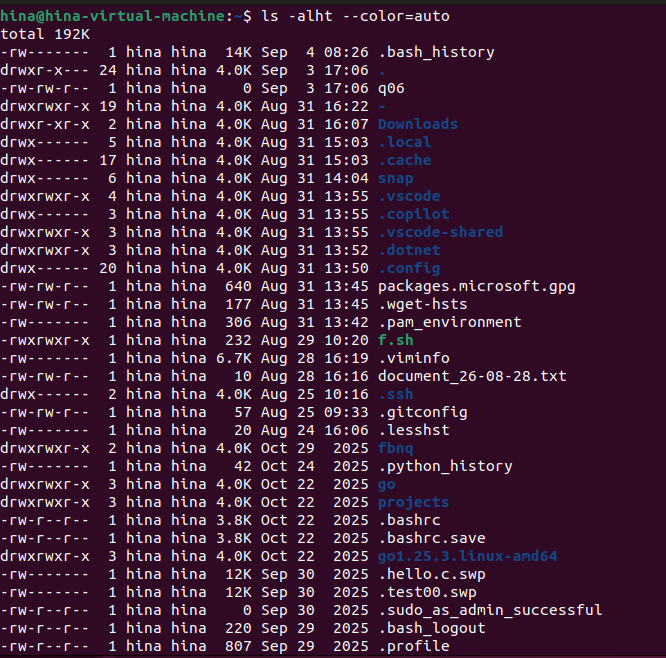
\includegraphics[width=15cm]{Q11.png}\\[0.3cm]\\

\subsection{第2题}
\label{sec:Q12}
\subsection*{题目内容}
假设你有一个很少失败的命令。为了调试它，你需要把它的输出保存下来，但等到一次失败运行可能会很耗时。
\begin{enumerate}
    \item 写一个bash脚本，不断运行下面这个脚本直到它失败为止
    \item 把标准输出和标准错误分别保存到文件里
    \item 把结果打印出来
\end{enumerate}

\subsection*{实现过程}
\begin{lstlisting}[language=bash, caption=使用到的代码]
CMD="./test.sh"

TMP_OUT="stdout.tmp"
TMP_ERR="stderr.tmp"
FINAL_OUT="stdout.log"
FINAL_ERR="stderr.log"

count=0

while true; do
    ((count++))
    $CMD > "$TMP_OUT" 2> "$TMP_ERR"
    exit_code=$?

    if [ $exit_code -ne 0 ]; then
        mv "$TMP_OUT" "$FINAL_OUT"
        mv "$TMP_ERR" "$FINAL_ERR"

        echo "Times: $count 次后失败 Exit Coed: $exit_code"
        echo "-------------------- stdout --------------------"
        cat "$FINAL_OUT"
        echo "-------------------- stderr --------------------"
        cat "$FINAL_ERR"
        echo "================================================="
        break
    fi
done
\end{lstlisting}
截图如下，同时stderr.log和stdout.log中均有对应内容\\
\includegraphics[width=10cm]{Q12.png}\\[0.3cm]\\

\subsection{第3题}
\label{sec:Q13}
\subsection*{题目内容}
\begin{enumerate}
    \item 终端里启动一个 sleep 10000 任务，用 Ctrl-Z 把它挂起，再用 bg 让它继续在后台运行。
    \item 使用 pgrep 找到它的 pid，再用 pkill 把它杀掉。
\end{enumerate}

\subsection*{实现过程}
\begin{lstlisting}[language=bash, caption=使用到的代码]
sleep 10000
#按下 Ctrl+Z，进程被挂起。
bg
pgrep -af "sleep 10000"
pkill -f "sleep 10000"
#确认进程杀掉
pgrep -af "sleep 10000"
\end{lstlisting}
过程截图如下\\
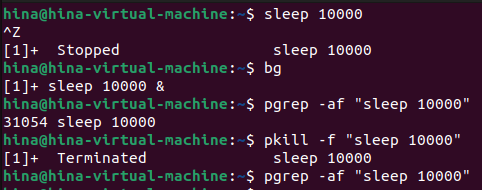
\includegraphics[width=10cm]{Q13.png}\\[0.3cm]\\

\subsection{第4题}
\label{sec:Q14}
\subsection*{题目内容}
\begin{enumerate}
    \item --是一个特殊参数--后面的所有内容都会被当作位置参数。
    \item 试着运行 touch -- -myfile，然后在不使用 -- 的情况下把它删掉。
\end{enumerate}

\subsection*{实现过程}
\begin{lstlisting}[language=bash, caption=使用到的代码]
touch -- -myfile
ls -l #确认文件存在
rm ./-myfile
\end{lstlisting}
截图如下\\
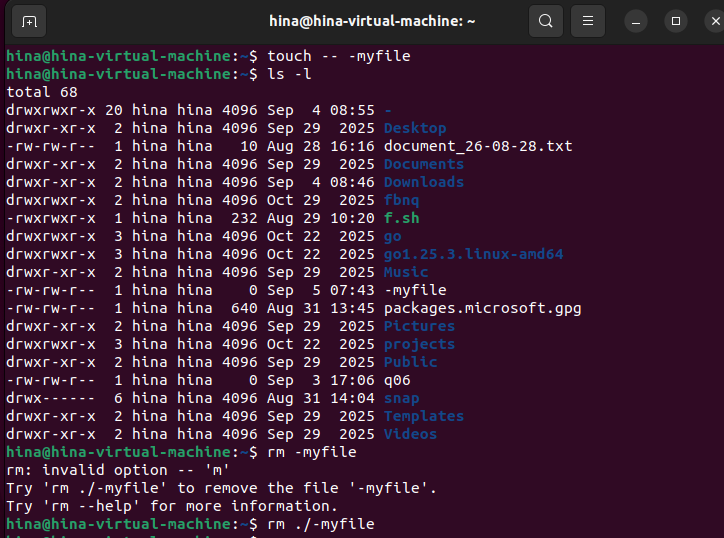
\includegraphics[width=10cm]{Q14.png}\\[0.3cm]\\

\subsection{第5题}
\label{sec:Q15}
\subsection*{题目内容}
\begin{enumerate}
    \item 试着配合 diff 和进程替换，比较 printenv 与 export 的输出。它们为什么不一样？
\end{enumerate}

\subsection*{实现过程}
\begin{lstlisting}[language=bash, caption=使用到的代码]
diff <(printenv | sort) <(export | sort)）
\end{lstlisting}
截图如下\\
printenv 和 export 输出不一样，是因为输出格式不同：printenv 用于机器解析，export 用于 shell 重新导入，因此包含声明关键字和引用处理。\\
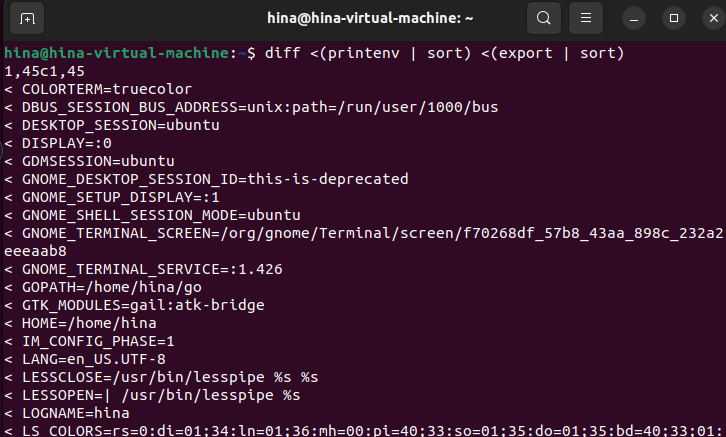
\includegraphics[width=10cm]{Q1501.png}\\[0.3cm]\\
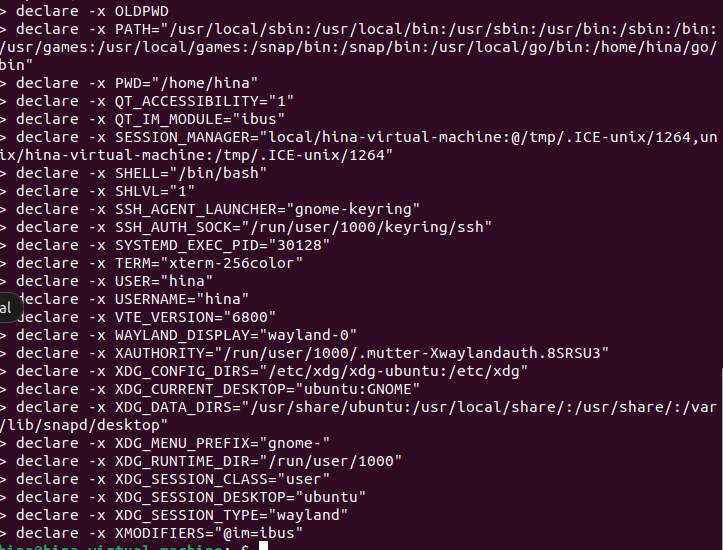
\includegraphics[width=10cm]{Q1502.png}\\[0.3cm]\\

\subsection{第6题}
\label{sec:Q16}
\subsection*{题目内容}
\begin{enumerate}
    \item 写两个 bash 函数 marco 和 polo
    \item 每次执行 marco 时，都要以某种方式保存当前工作目录；之后无论你切到哪个目录，只要执行 polo，它都应该把你 cd 回执行 marco 时所在的目录。
    \item 为了方便调试，你可以把代码写进 marco.sh，然后通过执行 source marco.sh 把这些定义重新加载到当前 shell。
\end{enumerate}

\subsection*{实现过程}
\begin{lstlisting}[language=bash, caption=使用到的代码]
#!/bin/bash

# 保存当前工作目录到变量 MARCO_DIR
marco() {
    export MARCO_DIR="$(pwd)"
    echo "Saved directory: $MARCO_DIR"
}

# 切换回保存的目录
polo() {
    if [ -n "$MARCO_DIR" ]; then
        cd "$MARCO_DIR" || echo "Failed to cd to $MARCO_DIR"
        echo "Now in: $(pwd)"
    else
        echo "Error: No directory saved. Run 'marco' first."
    fi
}
\end{lstlisting}
截图如下，可以看到在Q16文件夹使用marco后切换目录使用polo就切换回去了。\\
\includegraphics[width=10cm]{Q16.png}\\[0.3cm]\\

\subsection{第7题}
\label{sec:Q17}
\subsection*{题目内容}
\begin{enumerate}
    \item 你不想在某个进程完成之前启动另一个进程，限制条件始终是 sleep 60 \&。
    \item 一种实现方式是使用 wait 命令。试着启动这个 sleep，然后让一个 ls 等到后台进程结束后再执行。
\end{enumerate}

\subsection*{实现过程}
\begin{lstlisting}[language=bash, caption=使用到的代码]
sleep 60 &          # 启动后台任务
pid=$!              # 获取该任务的进程 ID
wait $pid           # 只等待这个特定进程结束
ls   
\end{lstlisting}
截图如下，可以看出输入的ls在sleep结束之后被执行\\
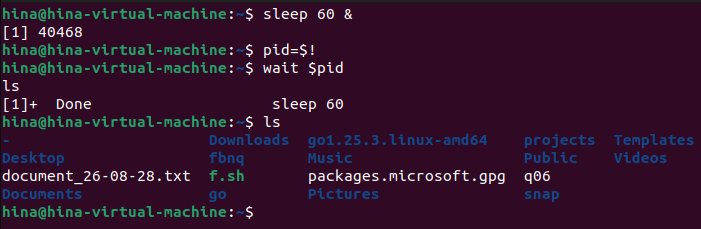
\includegraphics[width=10cm]{Q17.png}\\[0.3cm]\\

\subsection{第8题}
\label{sec:Q18}
\subsection*{题目内容}
\begin{enumerate}
    \item 按“最近修改时间”列出所有文件
\end{enumerate}

\subsection*{实现过程}
\begin{lstlisting}[language=bash, caption=使用到的代码]
find ~/- -type f -printf '%T@ %p\n' | sort -rn | cut -d' ' -f2-
\end{lstlisting}
截图如下，搜索的是我的git本地仓库，可以看见文件加入的顺序\\
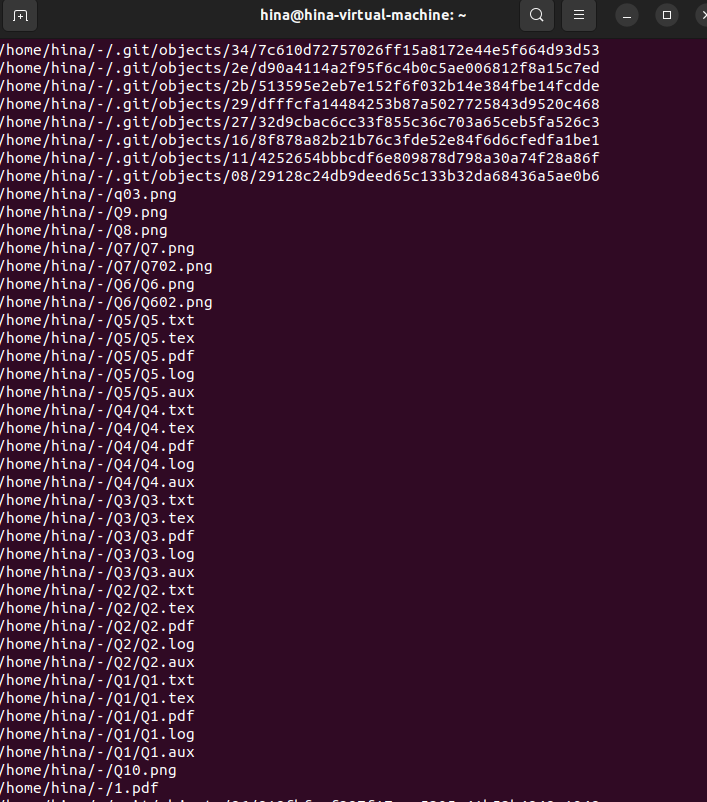
\includegraphics[width=15cm]{Q18.png}\\[0.3cm]\\

\subsection{第9题}
\label{sec:Q19}
\subsection*{题目内容}
\begin{enumerate}
    \item 执行以启动一个最小的网络服务器，位于4444端口。在另一个终端上运行以查找进程。用来终止。
\end{enumerate}

\subsection*{实现过程}
\begin{lstlisting}[language=bash, caption=使用到的代码]
#terminal 1
python -m http.server 4444
#terminal 2
ss -tlnp | grep 4444    
kill 41124
\end{lstlisting}
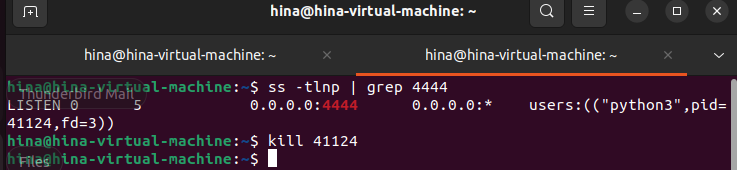
\includegraphics[width=15cm]{Q19.png}\\[0.3cm]\\

\subsection{第10题}
\label{sec:Q20}
\subsection*{题目内容}
\begin{enumerate}
    \item 创建一个 alias dc，让你把 cd 打错时也能正常工作。
\end{enumerate}

\subsection*{实现过程}
\begin{lstlisting}[language=bash, caption=使用到的代码]
echo "alias dc='cd'" >> ~/.bashrc
source ~/.bashrc
\end{lstlisting}
每次打开终端都自动加载该别名，效果如下：\\
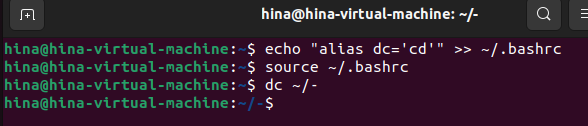
\includegraphics[width=15cm]{Q20.png}\\[0.3cm]\\

% ============================================================
% 个人感想
% ============================================================
\newpage
\section*{个人感想}
\addcontentsline{toc}{section}{个人感想}
通过本次实验，我对 Linux 命令行、调试器及性能分析工具的实际运用有了更直观的体会，尤其是在定位问题根源和进行针对性优化方面积累了经验。这些工具链的熟练使用，将为我今后的开发与调试工作提供扎实的支持。



% ============================================================
% 总结
% ============================================================
\section*{总结}
\addcontentsline{toc}{section}{总结}

\begin{conclusionbox}
本次实验完成了四项独立任务及十道综合练习题，覆盖了以下核心技能：
\begin{enumerate}
\item Shell 任务控制：掌握 bg、jobs、kill 及 PID 获取，理解前台/后台/挂起状态转换；
\item 语言服务器应用：使用 VSCode + Python 插件实现跳转、引用查找和全局重命名，熟悉 Ruff 静态检查；
\item 调试与缺陷修复：利用断点调试定位归并排序中的索引错误，并通过 pytest 增加回归测试；
\item 性能分析与优化：借助 cProfile 识别时间复杂度瓶颈，通过数据结构替换将词频统计速度提升约 8 倍；
\item 扩展 Shell 技巧：包括别名、进程替换、wait 同步、find 排序、网络服务控制等，丰富了日常开发工具箱。
\end{enumerate}
所有任务均基于 Linux 环境完成，并通过 Git 进行版本管理。本次实验不仅强化了基础工具链的使用，也培养了系统化排错和性能调优的工程素养。
\end{conclusionbox}

\end{document}